\chapter{Research Context}
Highly automated driving is currently an immensely attractive field for both academic and industrial research groups. 
A fully autonomous vehicle, which is able to tackle challenging driving situations without external input comparable to a human driver's performance, is yet to be build.
In this thesis, we propose a novel approach to knowledge and information representation for automotive environment models using cognitive modelling techniques.
More precisely, we adopt \acfp{VSA}, which are commonly used in tasks like cognitive modelling and natural language processing, for the specific application of automotive environment modelling.
To our knowledge, \acp{VSA} have not been applied in this particular context. 
In order to put our work in context of the current research landscape and to circumscribe this thesis, we need to review related work from several different areas like automated driving and mobile robotics, computational neuroscience, artificial intelligence and neuromorphic engineering.
A comprehensive overview for all of these research areas is out of scope of a single thesis.
However, we aim to cover the most significant results from all areas at least briefly, whereas we present an in-depth review of relevant work related to the thesis at hand, where necessary.

\section{Neuromorphic Systems}
To fully understand biological systems like the brain, which evolved over millions of years, is an ongoing yet unsolved challenge in biology and neuroscience.
Even small animals like insects or rodents show remarkable behavioural flexibility and the ability to constantly adapt to a rapidly changing and noisy world, which is unmatched by modern computing machines.
Mammals and primates are able to perform more sophisticated behaviours culminating in complex cognitive computations humans are capable of doing like thinking, problem solving, memory, reasoning, decision making, strategic planning, knowledge representation, learning etc.
The "biological computer" enabling these behaviours and cognitive abilities is the brain consisting of large networks of neural cells (or neurons), which communicate by sending and receiving electric signals via synapses.
At the same time, brains are comparably small and efficient: the human brain for example consumes only \SI{20}{\watt} of power (equivalent to a compact fluorescent light bulb) and comprises \SI{2}{\percent} of the body weight \cite[Chap. 2.1]{Eliasmith2013}. \\
Several research fields like computational neuroscience, neuromorphic engineering and neurorobotics try to reverse engineer biological systems to achieve similar performance and computational power.
During the last decades, researchers and engineers strived to close the gap in performance and efficiency between biological and artificial computing systems by mimicing neuro-biological architectures in hardware and implementing models of neural systems in software.
This biologically inspired, \textit{neuromorphic} approach promises not only to perform computations in a more efficient way, but also to tackle problems unsolvable with current computing machines.
\subsection{A brief history}
\begin{figure*}[t!]
	\centering
	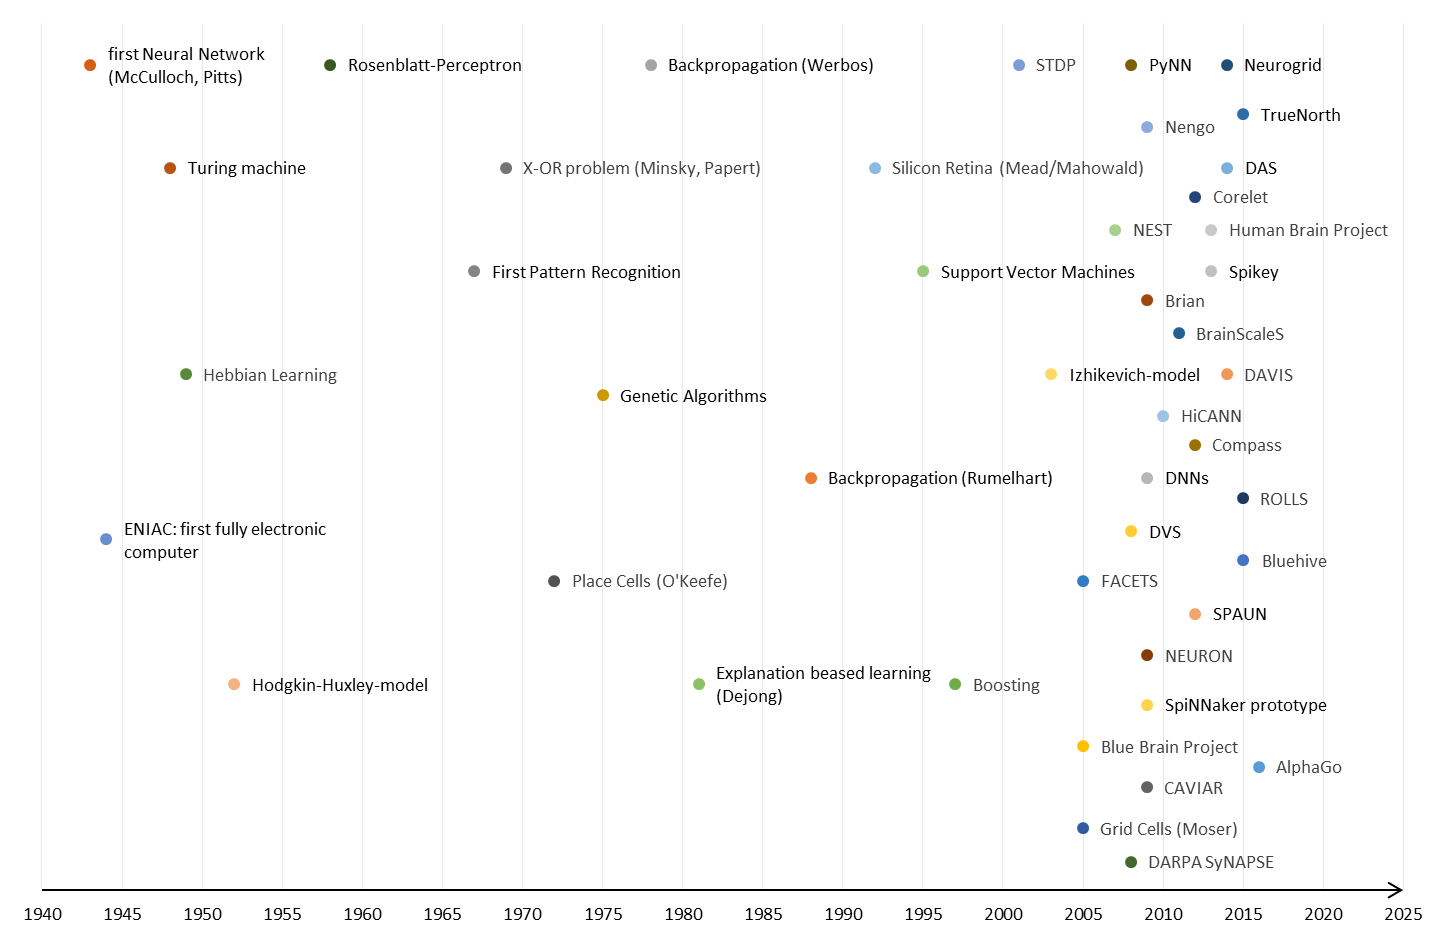
\includegraphics[width=0.95\textwidth,height=270px, natwidth=944,natheight=350]{imgs/Neuromorphic_Timeline_alpha.png}
	\caption{Historical developments in computational neuroscience, neuromorphic engineering and machine learning.\todo{check and possibly update this figure}}
	\label{fig:neuro_time}
\end{figure*}

The term neuromorphic itself was first introduced by Carver Mead in the late 1980s \cite{Mead90}, when describing one of the first silicon retinas.
He called artificial systems that share organization principles with biological nervous systems neuromorphic.
An interesting prototype of a silicon retina, which is now considered a milestone, was implemented by Misha Mahowald, a PhD student of Carver Mead. 
Her thesis received Caltech's Milton and Francis Clauser Doctoral Prize for its originality and potential for opening up new avenues of human thought and endeavor.
Since these early days of neuromorphic engineering, the term has widely been used to describe \ac{VLSI} systems \cite{Mead1989}, novel computing devices \cite{Schemmel2010}, sensory systems \cite{Lichtsteiner2008, Liu2010}, software \cite{Davison2008, Bekolay2014} and algorithms \cite{ReverterValeiras2016}.
Considering the number of scientists, neuromorphic engineering is still a comparably young field of research but received an increased interest during the last decade from both academic and industrial research groups caused by the funding of large, ambitious projects.
Although there have been several achievements in the field during the 1990s \cite{Mead1989, Mahowald1992, Indiveri1997, Cauwenberghs1998} and early 2000s \cite{Liu2002}, the \ac{FACETS} project \cite{FACETS-proj} and the \ac{BBP} \cite{BlueBrain-proj}, both starting in 2005 and mainly funded by the \ac{EU} under the FP6-\ac{FET} program, were among the first big-budget neuromorphic projects.
The follow-up project \ac{BrainScaleS} \cite{BrainScaleS-proj, Schemmel2010} (2011-2015) built on and extended the research conducted during the \ac{FACETS} project. 
The main developments of the \ac{FACETS} and \ac{BrainScaleS} projects are the \ac{HICANN} chip \cite{Schemmel2010} and the Python-based simulator-independant language \ac{PyNN} \cite{Davison2008} for building neural network models.
Building on \ac{BBP} the \ac{BrainScaleS} hardware development is currently continued in the neuromorphic computing platform of \ac{HBP} \cite{HBP-proj, Calimera2013}, a large ten-year research project, which was selected as one of the two \ac{EU}-\ac{FET} flagships in 2013 and is granted around one billion euros funding.
Another project starting in 2005, initially funded by the UK government until 2014 and now also part of the neuromorphic computing platform of \ac{HBP}, is the \ac{SpiNNaker} project \cite{Furber2014} during which the neuromorphic computing hardware of the same name was developed.
The \ac{HBP} is organized in thirteen platforms in total, which focus on different research fields related to the brain like for example theoretical neuroscience, neurorobotics, cognitive architectures, high performance computing, brain simulation and the aforementioned neuromorphic computing platform (see \cite{HBP-proj} for details).\\
Beside these research activities in Europe, the \ac{DARPA} funded another big-budget neuromorphic project: the \ac{SyNAPSE} program \cite{SYNAPSE-proj, Srinivasa2012}, which started in 2008 and is scheduled to run until 2016, has received 102.6 million US dollars in funding as of January 2013. 
The program aims to build an electronic microprocessor system that matches a mammalian brain in function, size, and power consumption.
Achievements during the \ac{SyNAPSE} program, which is primarily contracted to IBM Research and \acs{HRL}, so far are include brain simulations, design of brain-inspired neuromorphic achitectures \cite{Nere2012} and the development of a digital neurosynaptic core \cite{Merolla2011}, which is a building block of IBM's recently published TrueNorth chip \cite{Akopyan2015}.
Further project results are the Corelet language \cite{Amir2013} and the simulator Compass \cite{Preissl2012}, which enable dedicated software development as well as simulation and testing of TrueNorth algorithms on standard hardware respectively.\\
Beside these projects, the neuromorphic community is coming together at two annual (three- resp. two-week) workshops in Telluride and CapoCaccia, which have been established in 1994 and 2007 respectively, to discuss the current state of research in lectures and interactive talk sessions, to forge new ideas and to work on hands-on projects in small workgroups.

%----------------------------------------------------------------------------------------------------------
\subsection{\aclp{SNN}}
\label{subsec:SNN}
%----------------------------------------------------------------------------------------------------------
\begin{figure}[t!]
	\centering
	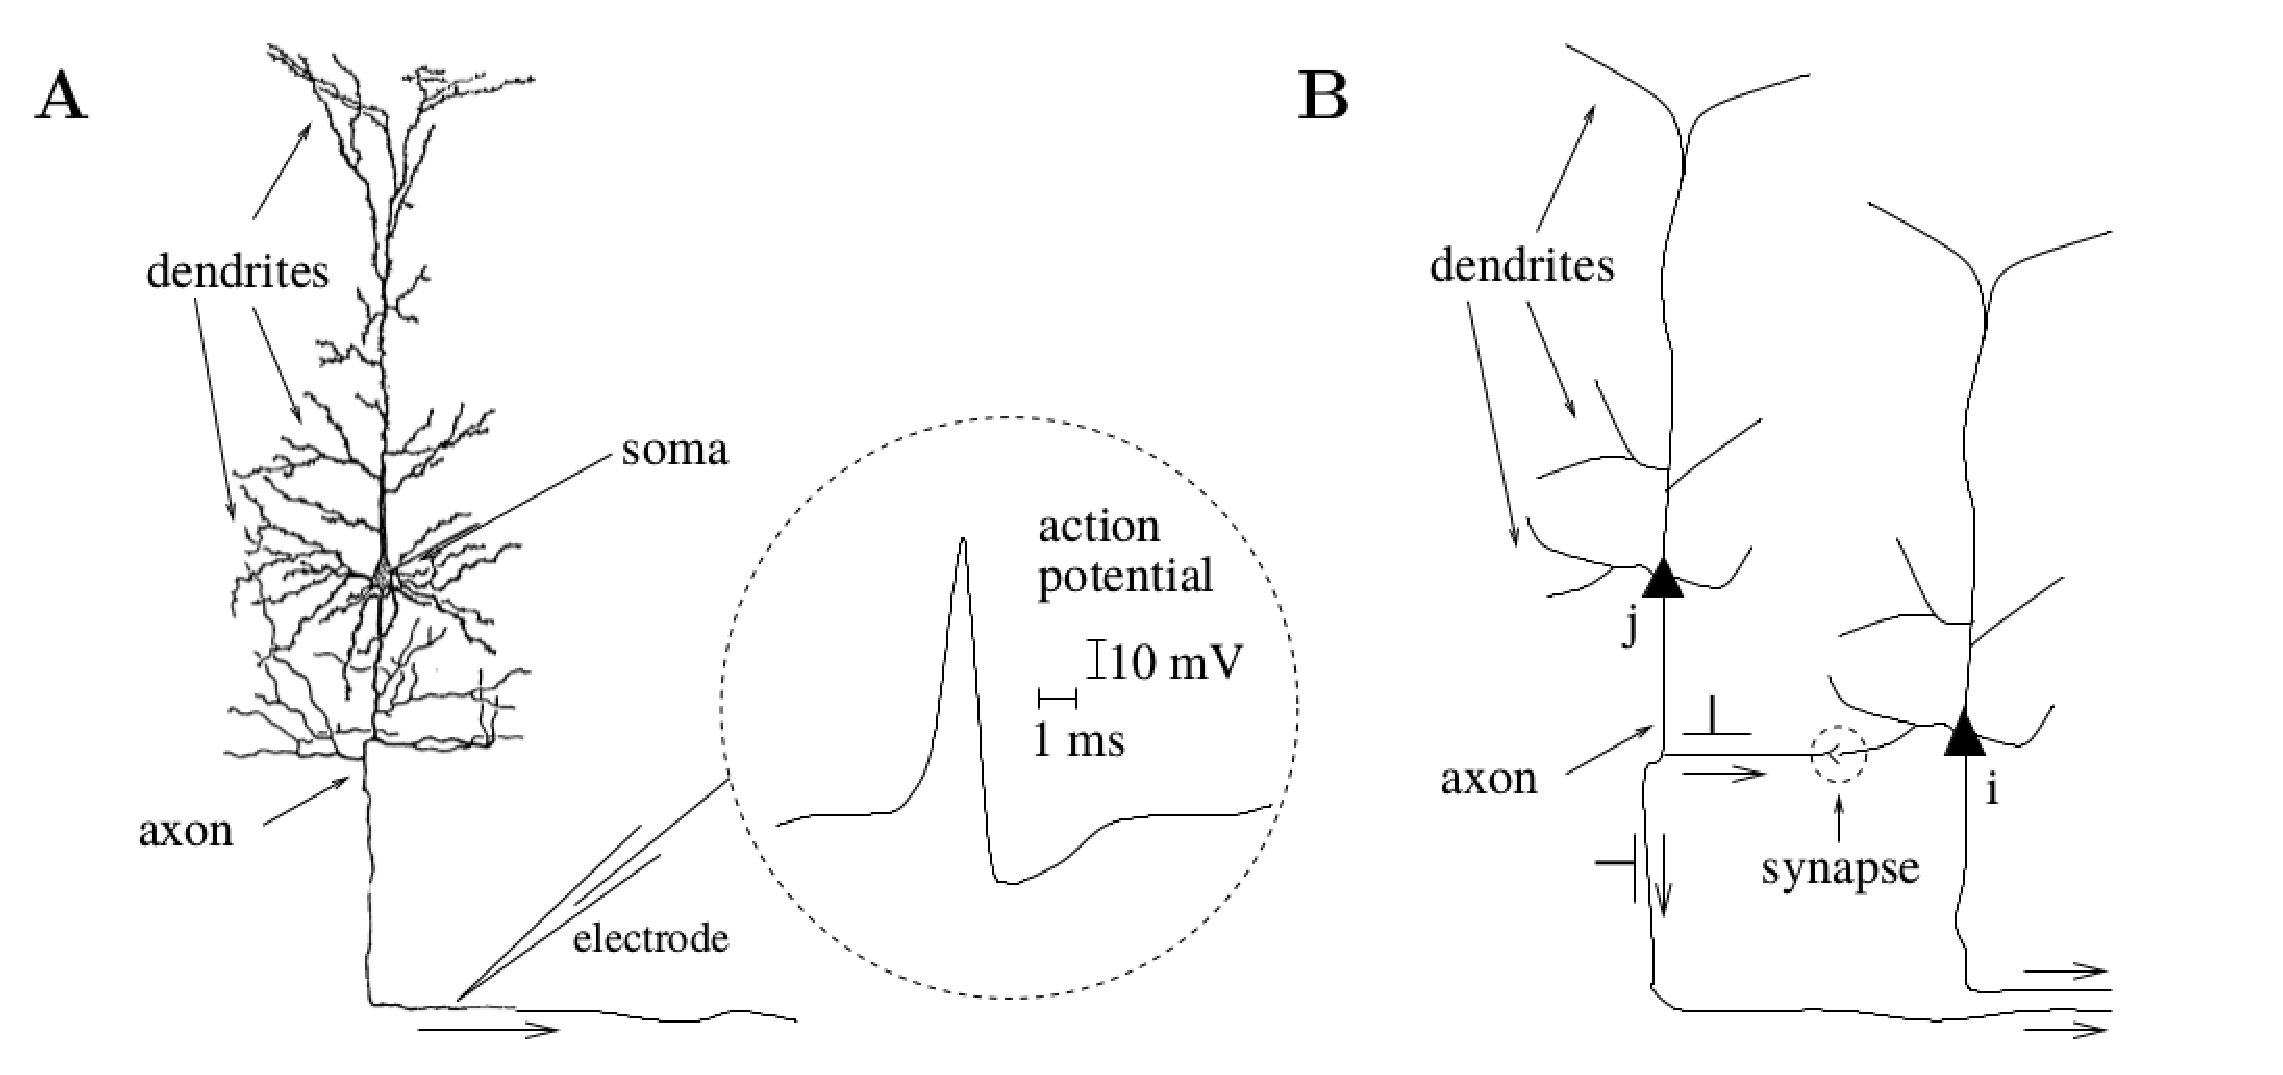
\includegraphics[width=0.85\textwidth]{imgs/Neuron_model.eps}
	\caption{Neuron visualization. Image source \cite{Gerstner2002}}
	\label{fig:biological_neuron}
\end{figure}
Biological neurons exchange information by sending short and sudden pulses, so-called action potentials or spikes.
\todo{include some text here referring to fig \ref{fig:biological_neuron}}
Whenever the membrane potential of a neuron, which can be in- or decreased by incoming spikes depending on the synaptic weight, reaches a certain threshold, the neuron produces a spike itself and resets its membrane potential afterwards \cite{Gerstner2002, Paugam2009}.
Recent neuroscientific research suggests that the exact timing of those spikes encodes information rather than just average firing rates \cite{Bohte2004}.
While traditional \acp{ANN} used in machine learning neglect these biological details, \acp{SNN} embody these spike times and are therefore often referred to as the third generation of neural networks \cite{Maass1997, Paugam2009}.
Maass showed in \cite{Maass1997}, that \acp{SNN} have at least the same computational power as threshold and sigmoidal neural networks of similar size.\\
The simplest spiking neuron model is the \acf{LIF} model with 
\begin{equation}
\frac{\partial V}{\partial t}(t) = - \frac{1}{\tau_{m}} \left( V\left(t\right) - R \cdot I\left(t\right) \right)
\label{eq:LIF}
\end{equation}
\begin{figure}
	\centering
	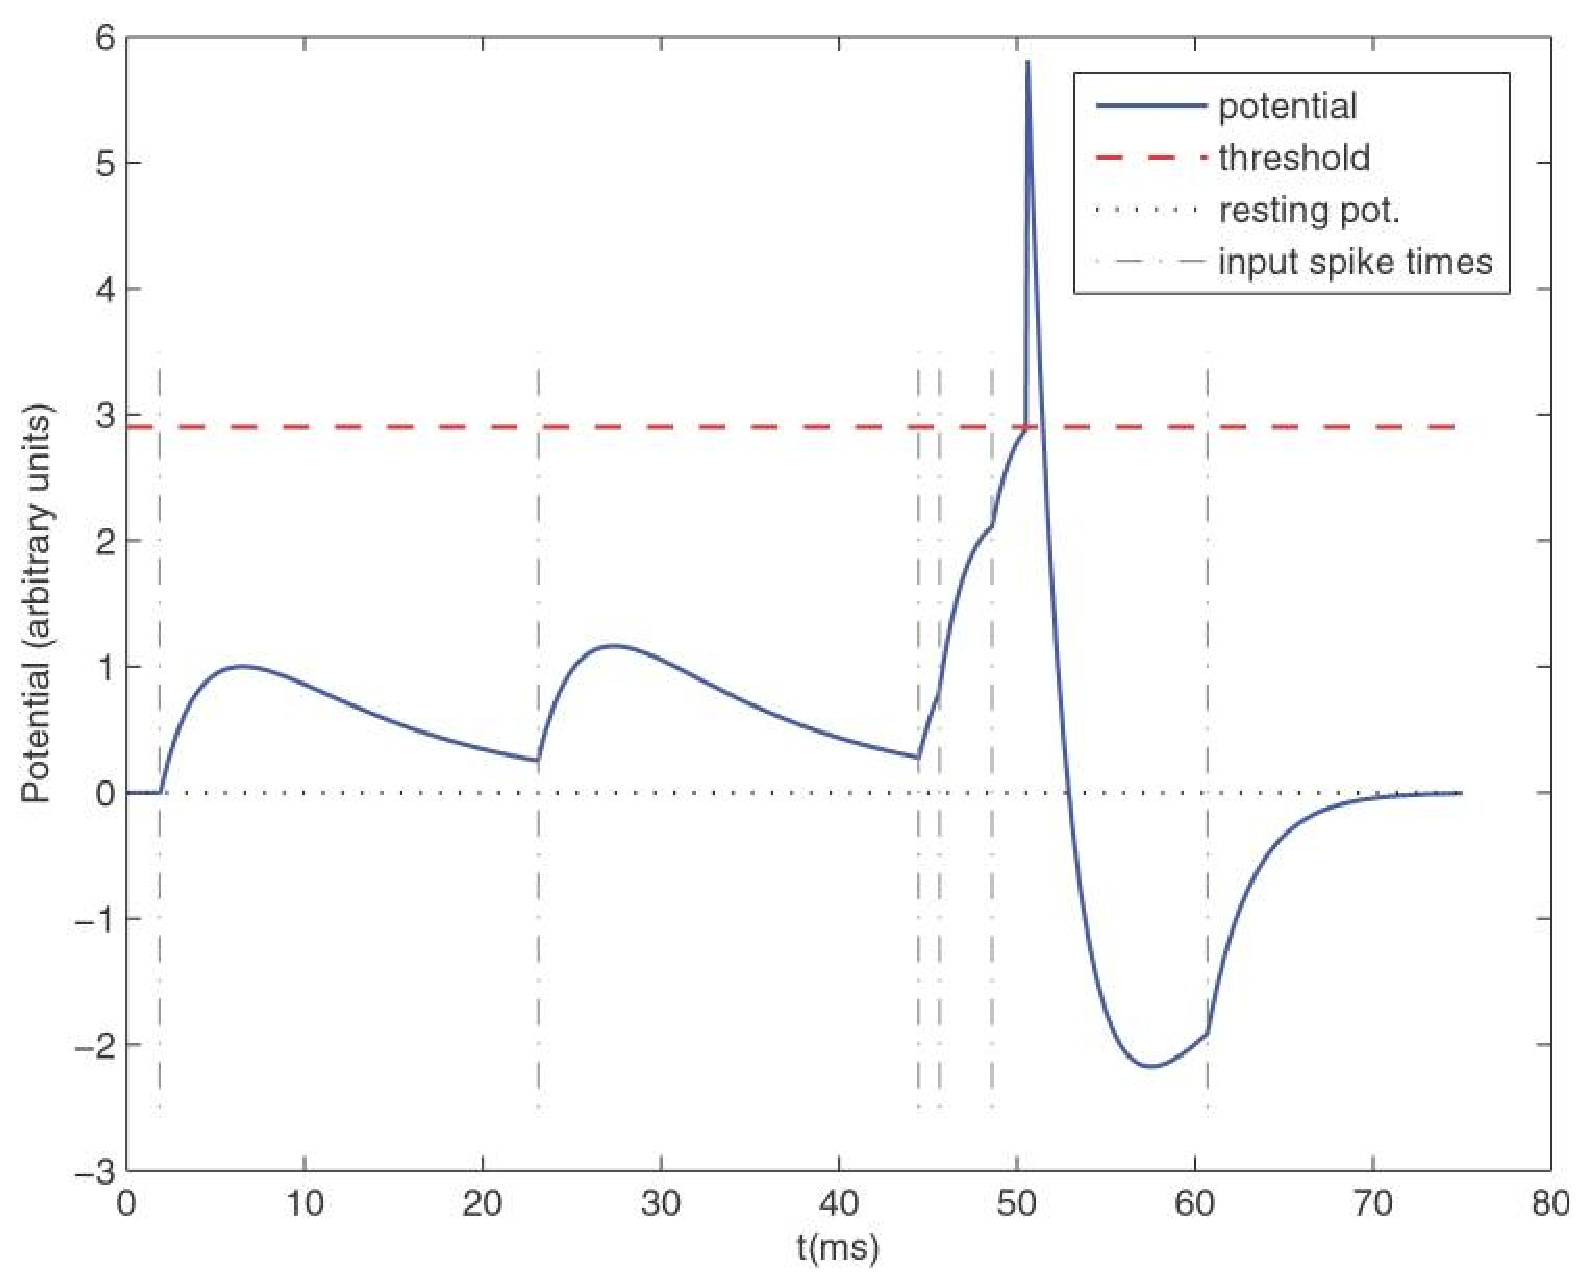
\includegraphics[width=0.75\textwidth]{imgs/LIF_Neuron.eps}
	\caption{Neuron visualization. Image source \cite{Masquelier2007}}
	\label{fig:lif_neuron_model}
\end{figure}
describing the subthreshold behaviour of the neuron, where $V$ is the voltage across the membrane, $I(t)$ is the input current, $R$ is the passive membrane resistance and $\tau_{m}$ is the membrane time constant.
Simply put, equation \ref{eq:LIF} states as follows: the membrane voltage increases in the presence of input current $I(t)$ depending on the membrane resistance $R$ while at the same time, especially in the absence of input current ($I(t)=0$), the voltage decreases or "leaks out" depending on the membrane time constant $\tau_{m}$.
When the voltage $V(t)$ passes a certain threshold $\vartheta$, the neuron produces a spike and the voltage is reset to a resting state $c$ for a certain refractory time interval $\tau_{ref}$ during which incoming spikes have no impact on the membrane potential.
Figure \ref{fig:lif_neuron_model} shows an an example curve of the membrane potential of one \ac{LIF} neuron based on six incoming spikes and visualizes the previously described behaviour. \todo{wording?}
The \ac{LIF} model, despite its biological simplifications, is maybe the most widely used neuron model for simulations due to its simplicity and comparably low computational complexity \cite{Izhikevich2004}, which allows simulations of large networks of neurons in reasonable time.
In contrast, the famous Hodgin-Huxley-model \cite{Hodgkin1952} with its four differential equations and dozens of (biologically meaningful) parameters is the model of high biological plausibility but also computationally challenging regarding large simulations \cite{Izhikevich2004}.
In 2003, Izhikevich proposed a neuron model \cite{Izhikevich2003} as compromise between biological plausibility and computational feasibility.
He showed that this simple model, described by two differential equations with four parameters, is able to produce all known spiking behaviours observed in cortical neurons \cite{Izhikevich2004}. \\
One major hindrance for the widespread adoption of \acp{SNN} has been the problem, that standard learning algorithms for traditional \acp{ANN} like backpropagation \cite{Werbos1974} can not be directly applied to \acp{SNN}.
Although an analogon, the so-called SpikeProp algorithm \cite{Bohte2002} for \acp{SNN} has been developed, the more natural approach is to transfer and mimic biologically inspired learning approaches like Hebbian learning \cite{Hebb1949} or \ac{STDP} \cite{Bi2001}.
An overview of several learning approaches for \acp{SNN} possibly applied with neuromorphic hardware can be found in \cite{Walter2015}.
Another possibility is to train a traditional \ac{ANN} and convert the resulting network into a \ac{SNN} \cite{Diehl2015, Hunsberger2015}.
An example for this approach is the network performing the visual digit recognition task as part of the larger \ac{Spaun} model \cite{Eliasmith2012}, which was derived by training a \ac{DNN} consisting of four \ac{RBM} layers and converting this network using the principles of the \ac{NEF} \cite{Eliasmith2003}.
Although theroretically superior \cite{Maass1997}, \acp{SNN} have not yet outperformed state-of-the-art \acp{DNN} in terms of accuracy in practical machine learning applications \cite{Schmidhuber2015}.\\
Beside the aforementioned procedures to solve traditional machine learning tasks with \acp{SNN} and thereby encode artificial functions in spiking neurons, a different approach is to try to understand how complex cognitive behaviours and the underlying neural functions are performed in the brain.
Therefore, the question how the brain encodes complex information and behaviour in trains of spikes and also how to decode these spike trains to reconstruct the encoded information needs to be answered. 
Although modern research has shed some light on this question regarding the neural code, it is still mainly unanswered as we do not fully understand the anatomical and neurophysiological processes within the brain \cite{Stanley2013}.
Currently, there exist several approaches to code information as spike trains, which can be summarized by the categories rate coding, temporal coding \cite[Chap. 7.6]{Gerstner2014}, population coding \cite[Chap. 1]{Gerstner2002}, \cite{Ponulak2011, Boerlin2011} or sparse coding \cite{Olshausen1996}.
Except for the biologically unrealistic rate coding approach, there are cues for all of these coding schemes and even combinations \cite{Gupta2014} of them to appear in biological systems.
\subsubsection{Software tools}
There exist several different programming languages, simulators and software libraries specifically designed for modelling \acp{SNN} varying from tools like Corelet \cite{Amir2013} and Compass \cite{Preissl2012} working with one specific hardware component, in this case IBM's TrueNorth chip \cite{Akopyan2015} (cf. Sec. \ref{sec:neuromorphic_HW}), to libraries like \ac{PyNN} \cite{Davison2008}, which aim for universality to work with different simulators and hardware components as back-end.\\
The simulation tool offering maybe the highest level of abstraction is \ac{Nengo} \cite{Stewart2009}, which implements the principles of the \ac{NEF} \cite{Eliasmith2003} and was used to build the \ac{Spaun} model \cite{Eliasmith2012}.
Originally written in Java, \ac{Nengo} was reimplemented in Python \cite{Bekolay2014} and improved by incorporating the lessons learned from the creation of \ac{Spaun}.
\ac{Nengo} allows the user to describe a model on a high level of abstraction by defining groups of neurons to simulate different functional blocks while \ac{Nengo} takes care of neural properties and synaptic weights using the \ac{NEF} (see Sec. \ref{sec:neural_eng} for more details).
\ac{Nengo} models can be run using the internal simulation back-end, but also simulation on some neuromorphic hardware components like Neurogrid \cite{Dethier2011, Choudhary2012} and \ac{SpiNNaker} \cite{Mundy2015}, which are currently used in developments aiming to run the \ac{Spaun} model in real-time, is supported.\\
Another Python-based tool is \ac{PyNN} \cite{Davies2010}, which was developed during the \ac{FACETS} \cite{FACETS-proj} and \ac{BrainScaleS} \cite{BrainScaleS-proj} projects and aims for building \ac{SNN} models independent of actual simulation tools. 
The level of abstraction is lower than \ac{Nengo}, but therefore it allows the creation of arbitrary neuron populations and connections, while the properties and synaptic weights need to be specified by the user or acquired using a learning algorithm.
\ac{PyNN} implements a number of standard models of neurons like \ac{LIF} or Izhikevich, connection algorithms like "one to one", "all to all" or connection matrices, static and plastic synapse types as well as several \ac{STDP} rules supported by the simulation and hardware back-ends.
Furthermore, \ac{PyNN} enables the user to implement custom models, connections and learning rules for advanced simulations and thereby extend the neural modelling toolkit.
\ac{PyNN} currently supports several different back-ends, e.g. simulators like \ac{NEST} \cite{Gewaltig2007}, Brian \cite{Goodman2009} and NEURON  \cite{Carnevale2009} as well as neuromorphic hardware.
\ac{PyNN} is currently the preferred development environment for the creation of \ac{SNN} models to run on the \ac{SpiNNaker} system \cite{Furber2014}.
The mapping of the network structure, neurons and synapses to actual cores on the chip is done with a separate software package called \ac{PACMAN} \cite{Galluppi2012}.\\
Another Python-based software package which, in contrast to \ac{PyNN} and \ac{Nengo}, mainly aims at modularity and flexibility in terms of supporting as many different neuromorphic hardware systems as possible as a front-end is \ac{PyNCS} \cite{Stefanini2014}.\\
A comprehensive overview of several other simulation tools for neural modelling can be found in \cite{Brette2007}.

%----------------------------------------------------------------------------------------------------------
\subsection{Neuromorphic Hardware}
\label{sec:neuromorphic_HW}
%----------------------------------------------------------------------------------------------------------

In this section, we give a brief overview of recent neuromorphic prototypes and hardware developments.
Although our work is not primarily targeted at use with this kind of dedicated hardware platforms, it shows promise regarding energy-efficiency and scalability in combination with specialized hardware components.
The neuromorphic prototypes described here are still comparatively young and not technologically mature yet, especially compared to traditional computing approaches.
Therefore, most of the hardware and sensors described are mainly developed and used in academia and are not standardized, commercial products yet. 
However, this technology is gradually becoming available to a broader community and draws increased attention in industrial research groups.

\subsubsection{Digital Neurochips}
\acp{GPU} provide a \ac{SIMD} architecture which helps in parallel data processing at the expense of large power consumption \cite{Krichmar2011, Carlson2014}. 
Due to fast matrix and vector multiplication capability of \acp{GPU}, at present they are providing an appealing platform for training and executing real-time data with the help of deep learning techniques \cite{Schmidhuber2015}. 
For specific applications, which take several months of training on a traditional \acp{CPU}, \ac{GPU}-based systems can accomplish the tasks in days \cite{Edwards2015}. 
A collaboration between NVIDIA and Stanford researchers demonstrated a cluster of \ac{GPU} servers which was able to train 1 billion parameters (scalable to 11 billion using 16 machines) on just 3 computers in two days. 
Each machine contained 4 NVIDIA GTX680 \acp{GPU} with \SI{4}{\giga\byte} at \SI{1}{\tera\nothing}\ac{FLOPS} each.\\
One of the recent developments in digital neuro-chips is IBM's TrueNorth \cite{Akopyan2015}. 
It contains a network of 4096 cores with 256 digital neurons each following a digital reconfigurable spiking neuron model \cite{Cassidy2013}, which makes over one million neurons and 256 million synapses in total consuming about \SI{65}{\milli\watt} of power. 
The cores are connected internally by a 2-D grid. 
The intersections of this grid contain routers which control the signal transmission within the network of cores inside a chip.
For programming this novel hardware implementation, a specialized programming language named Corelet was developed \cite{Amir2013}.\\
Another example of a digital neuromorphic hardware implementation is University of Manchester's \ac{SpiNNaker} Chip \cite{Furber2014}. 
It contains 18 synchronously connected ARM968 microprocessors and \SI{128}{\mega\byte} \ac{DDR} \ac{SDRAM}.
Communication is carried out by a packet-switched on-chip network, where all chips have a router.
This architecture scales well to larger application by allowing to place more chips on a board \cite{Painkras2013,Navaridas2009}. 
A \ac{SpiNNaker} system forms a toroidal mesh which has fixed connections, but the protocol implemented by the routers on the individual chips allows for the simulation of neural networks of arbitrary connectivity.\\
Another recent digital neuromorphic hardware platform is Intel's Loihi chip \cite{Davies2018}.
This chip consists of a fully asynchronous many-core mesh of $128$ neuromorphic cores, each containing $1024$ primitive units implementing spiking neuron behaviour in a tree-like strucutre.
In total, it contains $130000$ artificial spiking neurons and $130$ million synapses.
One of Loihi's key features is the ability of on-chip learning, which is realized through a learning engine integrated in each core that enables the implementation of learning rules to adapt parameters of the core's \ac{SNN}.

\subsubsection{Analog Neurochips}

Most of analog chips do not allow on-chip training due to limited adaptability of implementation techniques like capacitors \cite{Schwartz1990}, floating gate transistors \cite{Holler1990}, \acp{CCD} \cite{Agranat1990}. 
On the other hand, analog techniques use less components and offer high-speed operation. 
To exploit the benefits of analog semiconductor technologies and neural adaptivity, the learning algorithms have to be implemented on-chip. 
This, however, limits the reconfigurability of the platform and complicates the implementation of most learning rules directly into analog VLSI at the same time.
These limitations restrict the flexibility of analog designs compared to their digital counterparts. 
%They possess similar functional properties as that of biological networks and can be interfaced directly with real analog world \cite{Mead90}.\\
The \ac{HICANN} chip \cite{Schemmel2008} has the capability to simulate $131072$ synapses and $512$ neurons residing inside an \ac{ANC}. 
For simulation of large networks a wafer-scale integration method was used, which enabled $384$ \ac{HICANN} chips to be interconnected on a wafer of \SI{20}{\centi\meter} diameter \cite{Schemmel2010}. 
The spikes between various \acp{ANC} on a wafer or between interconnected wafers are carried out by a network of horizontal and vertical grid like structure. 
The horizontal pathway consists of 64 bus lines which carry spikes from 64 neurons. 
The 256 vertical lines collect spikes for all connected \acp{ANC}. 
The spikes are represented as data packet of 6-bits (for the group of 64-neurons) and transmitted using \ac{AER}. \\
The \ac{ROLLS} consists of $256$ neurons and $131072$ synapses. 
It consumes only \SI{4}{\milli\watt} of power and uses exponential \ac{IF} modelling \cite{Qiao2015}. 
The latest processor contains different configuration options. 
Each neural circuit is connected to three different types of synaptic circuits, first of which is an array of $256\times256$ synapse which can be excitatory or inhibitory. 
The synapses in the second $256\times256$ array offers only excitatory mode. 
In the third array, there are $256\times2$ virtual synapses whose weights are configurable with excitatory as well as inhibitory features. The virtual synapses operate in shared mode and occupy less space as compared to individual circuits. 
The neural spikes are generated and received using an \ac{AER} protocol with 8-bit neuron addresses \cite{Qiao2015}.\\
Another example of analog neural hardware is a chip \cite{Srinivasa2012} developed under \ac{DARPA}-funded \ac{HRL} \ac{SyNAPSE} project, which uses \ac{STM} for computation and memristors for synaptic weights storage. 
It contains a total of 576 neurons and 73728 synapses, arranged in an array of $24\times24$ neurons each with $128$ synapses and consumes \SI{130}{\milli\watt}. 
In \ac{STM} methodology a single synaptic circuit on the chip calculates multiple logical synapses of the simulated neural network because the electrical circuitry can function at much higher speeds than biological neurons. 
Hence a single synaptic circuit can emulate multiple logical synapses by switching between the corresponding parameter sets. 
There is a point-to-point routing mechanism hence no \ac{AER} is required \cite{Walter2015}. \\
The Brain in Silicon group at Standford University developed the custom board Neurogrid, which contains 16-Neurocores \cite{Benjamin2014, Choudhary2012}.
The neuron circuits are arranged in a 256$\times$256 grid, with every neuron has separate circuits for its soma and the dendrite. 
They combined analog computations with digital communication. 
The system is capable of simulating one million neuron and eight billion synapses in real-time and consumed \SI{3.1}{\watt} of power. 
The spikes are transmitted using \ac{AER}. 
It additionally implements a deadlock-free wormhole routing protocol to ensure free transmission of packets. 
It offers to explore different cortical areas of the brain by programming each of the Neurocores with a different model \cite{Merolla2014}. 

\subsubsection{Neuromorphic Sensors}
\label{subsubsec:neuro_sensors}
\begin{figure}[t!]
	\centering
	\subfloat[]{\label{subfig:DVS_rotationg_dot}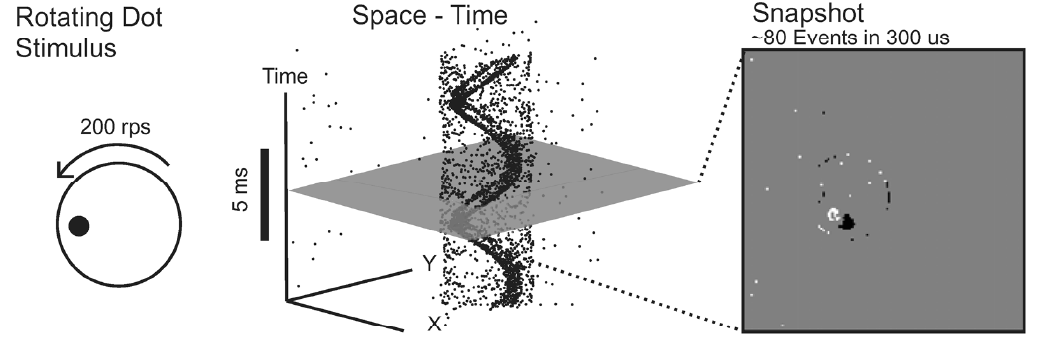
\includegraphics[width=0.9\textwidth,natwidth=944,natheight=624]{imgs/DVS_rotating_dot_stimulus.PNG}}
	\par\medskip
	\begin{minipage}{.48\columnwidth}
		\centering
		\subfloat[]{\label{subfig:DVS_pixel_core}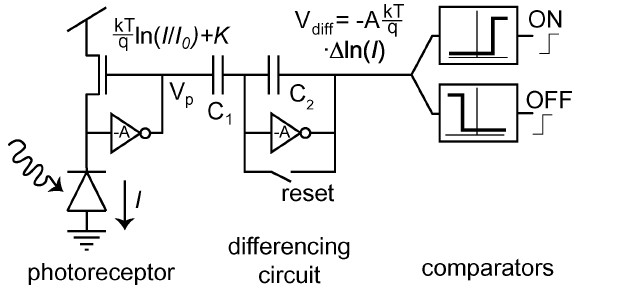
\includegraphics[width=1.15\textwidth,natwidth=944,natheight=624]{imgs/DVS_pixel_core.PNG}}
	\end{minipage}%
	\begin{minipage}{.48\columnwidth}
		\centering
		\subfloat[]{\label{subfig:DVS_operation_principle}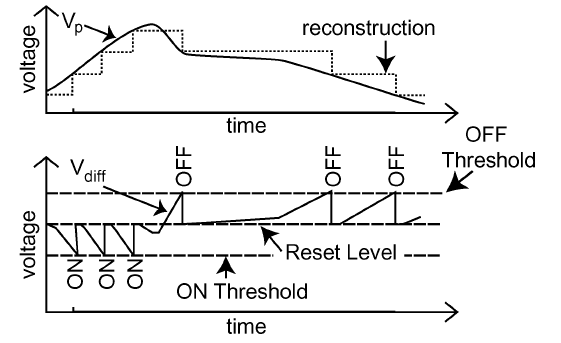
\includegraphics[width=0.9\textwidth,natwidth=944,natheight=624]{imgs/DVS_operation_principle.PNG}}
	\end{minipage}\par\medskip
	\caption{(a) Space-time representation of the event stream generated by a rotating dot on a spinning disk and a snapshot of the events (b) abstracted pixel core schematic (c) principle operation of single DVS pixel. Image source: \cite{Lichtsteiner2008}}
	\label{fig:DVS_with_schem}
\end{figure}
To adopt the neuromorphic hardware in real-world applications (e.g. neurorobotics), they need to be able to process sensors signals.
The neurally inspired, non von-Neumannian architecture requires either a new generation of sensors, e.g. the \ac{DVS} \cite{Lichtsteiner2008}, \ac{DAVIS} \cite{Brandli2014} or \ac{DAS} \cite{Liu2014}, which already embody the spiking neuron signal processing or a way of translating traditional sensor signals to sequences of spikes.
Several approaches to encode signals and stimuli with trains of spikes, e.g. by rate coding, temporal coding \cite[Chap. 7.6]{Gerstner2014} or population coding \cite[Chap. 1]{Gerstner2002}, \cite{Ponulak2011} have been investigated.
Neuromorphic sensors on the other hand, directly emit a sequence of events without the need of translation.
The \ac{DVS} for example, unlike traditional frame-based cameras, generates spike events \cite{Lichtsteiner2008} asynchronously for individual pixels when perceiving relative illumination changes (see Fig. \ref{fig:DVS_with_schem}), which are key features of biological vision \cite{Lichtsteiner2008}.
This event-based approach offers several advantages compared to conventional frame-based cameras like the ability to perceive very fast movements (sub-millisecond time precision) without the need to wait for and process the next frame as well as an output data rate depending on the dynamic content of the scene (Fig. \ref{subfig:DVS_rotationg_dot}) and thus reducing the output of redundant information.\\
The \ac{DVS}-pixels were designed to cover wide dynamic range and to offer low latency and mismatch. 
This is achieved by a fast photoreceptor circuit with logarithmic response whose output is fed into a high precision difference amplifier circuit followed by a two-transistor comparator circuit (see Fig. \ref{subfig:DVS_pixel_core} and \ref{subfig:DVS_operation_principle}). 
%The pixels are arranged in rows and columns which have $x$, $y$-address. 
The comparator circuit produces ON and OFF signals for each pixel, which are passed to the \ac{AER} interface for transmission via USB2.0 interface. \cite{Lichtsteiner2008}. 
On the other hand, the \ac{DAVIS} employs an \ac{APS} circuit to output synchronous global shutter frames, which helps in persevering absolute intensity information needed for classification and object recognition tasks while asynchronous \ac{DVS} events are beneficial for the tracking of fast movable objects \cite{Brandli2014}. 


\subsection{Neuromorphic Applications}
\label{subsec:neuro_applic}

In this section we present some examples of applications of neuromorphic hardware and sensors described in Sec. \ref{sec:neuromorphic_HW}, software, algorithms and neural modelling depicted in Sec. \ref{subsec:SNN} as well as combinations of both.
First, we describe applications using either neuromorphic sensors or hardware in combination with traditional computing hardware.
Then, we focus on purely neuromorphic systems, where the spiking signals of neuromorphic sensors, mainly the \ac{DVS}, is processed by neuromorphic hardware.
Although there are currently - to the knowledge of the author - no neuromorphic actuators working directly on the basis of spikes, we refer to the robotic systems described here as purely neuromorphic.


\subsubsection{Mixed systems}
\label{subsubsec:mixed_sys}

Neuromorphic vision \cite{Tan2015} is an emerging field of research, which aims to transfer approaches from traditional computer vision and also establish new methods incorporating the characterstics of the \ac{DVS}.
To perform pattern recognition tasks with neuromorphic cameras and at the same time use traditional methods as a benchmark, existing image data bases like the \ac{MNIST} data set \cite{LeCun1998} are translated to neuromorphic datasets by presenting the images on a computer screen to a \ac{DVS} sensor moving minimally back and forth \cite{Orchard2015} (mimicing saccade movements of the human eye), which gives better results than moving the images themselves on the screen \cite{Serrano-Gotarredona2013}.\\
As the \ac{DVS} naturally captures moving objects when held statically and cues of the ego-motion when moving, tracking of these movements are suitable applications making use of the sensor's characteristics.
These characteristics along with the \ac{DVS}'s advantages compared to traditional frame-based cameras, which have been described in Sec. \ref{subsubsec:neuro_sensors}, have been demonstrated in applications like pencil balancing \cite{Conradt2009} and a robotic goalie \cite{Delbruck2013} interfacing the \ac{DVS} with traditional computing hardware and actuators. 
Keeping track of (geometric) features \cite{Lagorce2015} and contours \cite{Barranco2014} observed by the \ac{DVS} lays the foundation for more sophisticated algorithms.
Researchers recently proposed several approaches for tracking people \cite{Schraml2010, Piatkowska2012} and other geometric objects \cite{ReverterValeiras2016} using stationary sensors.
Especially tracking at high velocities \cite{Saner2014} benefits largely from the sub-millisecond time precision of the \ac{DVS} even enabling tracking of particles in fluid flows \cite{Drazen2011}, which would require a high-speed PC, lots of disk space and high-intensity laser strobe lighting to illuminate the fluid in a conventional setting.\\
A traditional application of computer vision in robotics is the estimation of the ego-motion or odometry based on optical flow (an event-based approach on optical flow can be found in \cite{Benosman2014}), which can also be obtained by combining traditional cameras with the \ac{DVS} on a small wheeled robot \cite{Censi2014}.
Another suitable application for the \ac{DVS} is the estimation and tracking of the whole six degree-of-freedom pose of a flying robot, especially when performing high-speed maneuvers, where traditional cameras suffer from motion blur \cite{Mueggler2014}.
Another problem in robotics closely related to tracking is self-localization of the robot using a given map of the environment or building a map online and localizing within this map at the same time, which is known as the \ac{SLAM} problem \cite{Thrun2005}.
Localization performed within a given map using the \ac{DVS} on ground vehicles and by tracking markers from a flying robot is presented in \cite{Gallego2015} and \cite{Censi2013} respectively. 
There are also several papers treating the \ac{SLAM} problem \cite{Weikersdorfer2012, Weikersdorfer2014} or the related problem of tracking the camera pose and simultaneously reconstructing the observed scene by mosaicing \cite{Kim2014} with neuromorphic vision sensors.\\
Most of the tracking algorithms mentioned here use variations of traditional Bayesian filters like (extended) Kalman- or particle-filters \cite{Thrun2005} for consecutive estimation of the quantity of interest.
However, due to the asynchronous information processing of the \ac{DVS} or neuromorphic systems in general these filters need some modifications to work with this event-based approach \cite{Weikersdorfer2013} like taking several past measurements into account (in contrast to the traditional Markov assumption) or updating only after a certain number of events have occurred to avoid computational overhead.\\
In \cite{Axenie2015}, the authors describe a biologically inspired system for sensor-fusion of several traditional sensors like wheel encoders, magnetometer and gyroscope for ego-motion estimation demonstrated in ground and flying robots.
Another example for sensor fusion is presented in \cite{OConnor2013}, where the biologically inspired \ac{DVS} and \ac{DAS} sensors are used to recognize hand-written digits from the \ac{MNIST} dataset \cite{LeCun1998}.
To incorporate the neuromorphic audio sensor, each digit is assigned one tone frequency in the A harmonic minor scale, while the actual fusion is performed by a \ac{DBN} consisting of several, pre-trained (unsupervised) \ac{RBM} layers, which was traditionally trained and afterwards transferred to an event-based network.
Although the authors state that the actual implementation in \cite{OConnor2013} is just a proof-of-concept in software, their approach shows promise to translate fully trained \acp{DBN} to \acp{SNN}, deploy them on efficient neuromorphic chips and thereby making this technology available for mobile and/or real-time applications.\\
To demonstrate the functionality and applicability of their neuromorphic chip TrueNorth, IBM implemented several proof-of-concept applications ranging from virtual robots, game simulations \cite{Arthur2012}, digit recognition \cite{Arthur2012, Esser2013} to classical machine learning tasks like object detection \cite{Akopyan2015}.
In \cite{Arthur2012} the authors present four example applications of neural algorithms implemented on TrueNorth using the Corelet language: a virtual robot driver aiming to keep the simulated robot on a virtual road based on visual cues, a neural algorithm controlling an autonomous player performing the classical video game pong, a neural implementation recognizing hand-written digits of the \ac{MNIST} data-base using \acp{RBM} as well as a Hopfield network, which performs autoassociation.
Seven example algorithms and applications for TrueNorth are presented in \cite{Esser2013}: speaker recognition using \acp{CNN} on the \ac{CUAVE} data set \cite{Patterson2002}, composer recognition distinguishing between classical composers Bach and Beethoven using liquid state machines, recognition of hand-written digits of the \ac{MNIST} data set using population coding and \acp{RBM}, a neural implementation of a \ac{HMM}, collision avoidance using motion extraction and looming detection, optical flow based on \acp{CNN} and eye detection using the \ac{DVS}.
Most of these algorithms are simplified proof-of-concept implementations showing the general applicability of TrueNorth but are not competitive with traditional machine learning algorithms yet (e.g. \SI{92.34}{\percent} \cite{Esser2013} vs. \SI{99.77}{\percent} \cite{Ciresan2012a} correct classifications on \ac{MNIST}).
In \cite{Schmitt2017}, the authors demonstrate training and deployment of \acp{DNN} on the \ac{MNIST}-dataset using the \ac{BrainScaleS} hardware.
A more sophisticated application is the multi object detection and classification task described in \cite{Akopyan2015}, which detects moving and stationary people, bicyclists, cars, buses and trucks from a HD video stream in real-time recorded by a stationary camera using Haar-like features, saccades, K-means- nd Grid-classifiers.\\
The use of the neuromorphic hardware Neurogrid \cite{Benjamin2014} as computational back-end for \ac{Nengo} and proof-of-concept solution for medical motor-protheses, which shall be connected to biological neurons and thereby be controlled by the patient's brain, is described in \cite{Choudhary2012} and \cite{Dethier2011} respectively.
The \ac{SpiNNaker} system \cite{Furber2014} also supports the simulation of neural models created using \ac{PyNN} or \ac{Nengo} \cite{Mundy2015}.
Furthermore, several neural network architectures like \acp{CNN} \cite{Serrano-Gotarredona2015} and pre-trained \acp{DBN} \cite{Stromatias2015, Stromatias2015a} have also been implemented on the \ac{SpiNNaker} system.\\
To enable biologically inspired learning like \ac{STDP} \cite{Bi2001}, according rules adapting the synaptic weights depending on the timing of the spikes have efficiently been implemented on the \ac{SpiNNaker} \cite{Diehl2014} chip as well.
\todo{include phrase about own omnibot paper \cite{Mirus2018a}}
\subsubsection{Purely neuromorphic systems}
\label{subsubsec:neuro_systems}

\begin{figure}[t!]
	\centering
	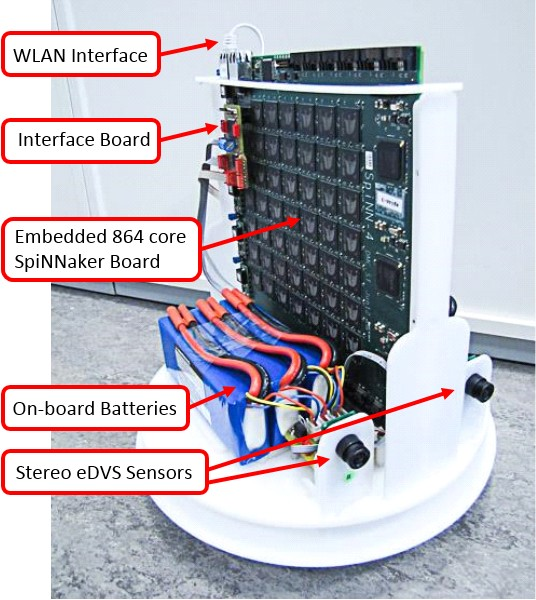
\includegraphics[width=0.48\textwidth,natwidth=944,natheight=624]{imgs/SpinRobot.jpg}
	\caption{Example of a closed-loop, neuromorphic robotic system with two event-based embedded \acp{DVS} and a 48-node \ac{SpiNNaker} board. Image source: \cite{Galluppi2014}}
	\label{fig:spin_robot}
\end{figure}
Some examples of closed-loop systems deployed in small robots are presented in \cite{Davies2010, Denk2013, Galluppi2014}. 
In \cite{Davies2010, Denk2013}, the authors interface two embedded \ac{DVS} cameras directly with a \ac{SpiNNaker} platform mounted on a small robot (see Fig. \ref{fig:spin_robot}). 
The implemented neural networks enable simple autonomous behaviours like following a line \cite{Davies2010} or approaching a light stimulus \cite{Denk2013}.
In \cite{Galluppi2014}, a small robot with a similar setup is able to perform trajectory stabilization using optical flow from the \ac{DVS} cameras as input.
Another simple task described in \cite{Galluppi2014} is the recognition and tracking of a light stimulus and keeping the robot at a certain distance and angular orientation with regard to this stimulus.
The whole processing chain from visual perception over internal processing to motor control in these robot experiments are realized using spiking neuron models.
The neural implementation of the latter two applications are done in \ac{PyNN} and \ac{Nengo} respectively.\\
While the aforementioned sensorimotor behaviours are manually engineered, there are attempts to learn more sophisticated, complex behaviours from simpler basic movements \cite{Conradt2014, Stewart2016}.
These basic maneuvers are still manually engineered relating sensor cues to simple movements like driving forward with no obstacle in the sensors field of view, turning with an obstacle in in front of the robot or driving backwards when being close to an obstacle.
In \cite{Conradt2014} the authors describe a method on learning more sophisticated behaviours from recorded sensorimotor data obtained from driving the robot by remote control as training examples, which can be considered as a supervised learning approach.
In \cite{Stewart2016}, the training examples are taken from recording data of the robot driving around without human interference and just labeling those situations as positive examples when the robot performed the desired action by accident, which is considered as reinforcement learning.
Both approaches are implemented on a small robot with the \ac{DVS} as sensory input using \ac{Nengo} and the \ac{NEF} as well as its interface \cite{Mundy2015} for running neural networks models on the \ac{SpiNNaker} hardware \cite{Furber2014}.
%----------------------------------------------------------------------------------------------------------
\section{\aclp{ANN}}
\label{sec:ML_ANN}
%----------------------------------------------------------------------------------------------------------
Machine learning in general is the science of constructing computer programs, which improve with experience. 
This is attractive if manually programming a desired functionality is not cost-efficient, intractable or simply impossible.  
The overall goal of machine learning algorithms is to generalize beyond examples, i.e. to generate models that describe the presented input sufficiently well to make the best possible prediction when confronted with previously unseen data.
A formal, widely cited definition of machine learning has been presented by Thomas M. Mitchell in \cite{Mitchell1997}:
\begin{defn}
	A computer program is said to \textbf{learn} from experience $E$ with respect to some class of tasks $T$ and performance measure $P$ if its performance at tasks in $T$, as measured by $P$, improves with experience $E$.
\end{defn}
A large body of research has focused on machine learning during the last decades.
One major branch of machine learning are \acp{ANN} and \acp{DNN} in particular, which are currently the state-of-the-art of many machine learning tasks.
\subsection{A brief history}
The research field of \aclp{ANN} goes back to the 1940s when McCulloch and Pitts introduced artificial neurons as computational units \cite{McCulloch1988}, which embody a simplified model of biological neurons.
These first simple networks were able to calculate compositions of basic logic functions \cite{McCulloch1988, Rojas1996}.
Rosenblatt \cite{Rosenblatt58} proposed the first neural network, which was capable of learning, by adding numerical weights to the connections of the network with threshold functions as activation functions: the \textit{perceptron}.
Minsky and Papert \cite{Minsky1969} showed, that single-layer perceptrons are not able to calculate an XOR-function or, more generally, are only capable of learning linearly separable patterns.
This caused a decreased interest in neural networks research until the rediscovery of the backpropagation algorithm \cite{Werbos1974} in the 1980s \cite{Rumelhart1988}, which introduced a practically feasible method to optimize the network weights using gradient descent and led to a resurgence of neural network research.
%This gradient descent called for continuous activation functions (mostly sigmoid or hyperbolic) instead of threshold-functions as activation functions, which made the so-called second generation \ac{ANN} universal approximators for continuous functions \cite{Cybenko1989}.
Since then, various different network architectures like feed-forward, \acp{CNN}, \acp{RNN}, \acp{RBF}, \acp{RBM}, \acp{SOM} and \ac{ART} just to name a few \cite{Schmidhuber2015} have been proposed for different learning paradigms.
Although several simpler methods like Boosting \cite{Freund1997} or \acp{SVM} \cite{Vapnik1995} have been developed and achieved noteworthy results, the availability of powerful, parallelized computing hardware like \acp{GPU} as well as the advent and success  of deep learning (partly achieving better-than-human accuracy) made \acp{ANN} \cite{Rojas1996} and especially \acp{DNN} \cite{LeCun2015} the state-of-the-art for several machine learning tasks like visual digit \cite{Ciresan2012a} and traffic sign \cite{Ciresan2012} recognition in recent years.
Another great achievement in the field of deep learning was the victory of AlphaGo \cite{Silver2016} over the world's best Go player Lee Sedol in March 2016, which was considered to be at least a decade away due to the complexity of Go.
Compared to Deep Blue, the system that beat former chess world champion Garri Kasparov in 1997 \cite{Hsu2002} with sheer computational power by brute forcing through a large number of possible moves in advance to find the best one, this strategy is not feasible for Go due to its higher complexity (larger board, more options to consider per move).
In contrast, modern \acp{DNN} trained by a combination of supervised learning from human expert games and reinforcement learning from self-play have been used for the evaluation of board positions and selection of moves to avoid expensive lookahead search \cite{Silver2016}.
A comprehensive and historical overview of relevant literature concerning \acp{ANN} and especially \acp{DNN} can be found in \cite{Schmidhuber2015, LeCun2015}.
\subsection{Supervised Learning}
\todo{brief introduction to \acp{DNN} in general, particularly \acp{CNN} for classification, mentioning automotive related applications. Also mention \acp{RNN} and especially \ac{LSTM} as for time-series analysis/prediction as it is related to our behaviour prediction task}
\subsection{Unsupervised Learning}
\todo{brief introduction some unsupervised learning strategies. Focus especially on approaches to learn word embeddings like word2vec \cite{Mikolov2013}, GloVe \cite{Pennington2014}. Also mention problems of those approaches \cite{Levy2015}}
\subsection{Reinforcement Learning}
\todo{very brief introduction. Not sure yet if we need this secton at all}
%From the first theoretical considerations concerning artificial neural networks by McCulloc and Pitts(\todo{Citation}) in the 1940s and the first Multilayer-Perceptrons by Rosenblatt (\todo{Citation}) about a decade later, machine learning algorithms started to receive widespread attention with the rediscovery \cite{Rumelhart1988} of the well-known backpropagation algorithm \cite{Werbos1974}.
%Since then, several approaches to machine learning, apart from artificial neural networks, like AdaBoost (\todo{Citation}), Decision Trees (\todo{citation}), Bayesian Networks (\todo{citation}) or \ac{SVM} (\todo{citation Vapnik, V. (1995), The Nature of Statistical Learning Theory. Springer Verlag, Cristianini, N. and Shawe-Taylor, J. (2000). An Introduction to Support Vector Machines and Other Kernel-Based Learning Methods. Cambridge University Press, Cambridge}) have been proposed.
%These methods vary in representation of the data, the evaluation (or objective) function, the optimization technique and the learning paradigm.
%Through availability of larger datasets and increased computational power, machine learning has seen significant progress in recent years.
%The use of deep neural networks \cite{Schmidhuber2015}, enabled through modern, powerful computing hardware like \ac{GPU}, yielded a significant performance boost in several classification tasks. 
%Today, modern deep learning algorithms can even rival human performance on different visual classification tasks like traffic sign \cite{Ciresan2012} or digit recognition \cite{Ciresan2012a}.
%
%So-called second generation \ac{ANN} introduced continuous (e.g. sigmoid or hyperbolic) instead of step- or threshold-functions (\todo{Citation}) as activation functions, which made them universal approximators for continuous functions \cite{Cybenko1989}.
%The term "neuromorphic" was first introduced by Carver Mead in \cite{Mead90}, when describing one of the first silicon retinas.
%For clarity, a first broad definition is provided, which will need some refinement while proceeding in this section:
%\begin{defn}
%\label{def:neuromorph}
%Artificial systems, that share organization principles with biological nervous systems are called \textbf{neuromorphic}.
%\end{defn} 
%Biologically inspired systems and algorithms have seen significant progress and achieved remarkable results, e.g. in the field of machine learning, despite some simplifications in terms of biological accuracy.
%So-called first and second generation \ac{ANN} described in \ref{subsec:ML_ANN} are also covered by definition \ref{def:neuromorph} as neuromorphic systems, although they neglect some biological details.
%\subsection{Spiking Neural Networks}
%Biological neurons exchange information by sending short and sudden increases in their membrane voltage, so-called action potentials or spikes.
%Recent neurological research suggests that the exact timing of those spikes encodes information rather than just average firing rates (\todo{Citation}).
%While \ac{ANN} of the first two generations neglect these biological details, recent neural networks structures, so-called \ac{SNN} \cite{Paugam2009}, embody these spike times and are therefor often referred to as the third generation of neural networks . 
\section{Automated Driving}
"Robotics is the science of building computer-controlled mechanical devises, which are able to perceive and manipulate the physical world" \cite{Thrun2005}.
Automated driving in automotive context is a special case of robotics, since an autonomous vehicle can be considered a wheeled mobile robot, which is able to fulfill the transportation capabilities of a traditional car without human input. 
In order to navigate safely to a desired goal, a mobile robot needs to solve several problems like localization ("where am I?"), path planning ("how do I get from A to B?"), environment perception ("where is everyone else?"), knowledge representation and reasoning ("which decisions to infer from available information?") as well as motion control ("how to move my actuators?").
In automotive context, an automated vehicle furthermore needs to detect the current state of the driver ("what is the driver up to") to ensure that he can take over control in safety-critical situations or in case of malfunctions.
The human driver as a fallback option in such situations is of crucial importance, since the level of driving automation gradually increases instead of a hard transition to automated driving systems.
In their J3016 standard \cite{SAE_J3016}, the \ac{SAE} delivers a classification system identifying six different levels of driving automation from "no automation" to "full automation".
Table \ref{tab:autonomy_levels} gives an overview of the particular automation levels according to \cite{SAE_J3016} in more detail.
\subsection{A brief history}
On the road to fully automated driving, several \ac{ADAS} have been developed during the last decades and thus made a huge jump by incrementally increasing complexity and therefor the level of autonomy.
The history of automated driving research goes back to the 1980's, when governmental institutions funded several explorative projects worldwide to research functionalities like automatic vehicle driving and intelligent route planning resulting in early prototypes.
In 1986, several European research groups and vehicle manufacturers started the \ac{PROMETHEUS} project \cite{Dickmanns1990} and demonstrated a variety of different approaches to automated driving.
Another research initiative established during that period is Carnegie Mellon University's Navlab \cite{Thorpe1988}, which achieved the first completely autonomous drive from Pittsburg to San Diego.
After that first explorative phase, the US government established the \ac{NAHSC} in 1995 and shortly shortly followed by the foundation of the \ac{AHSRA} 1996 in Japan.
The main contribution of this first phase was the identification and deep analysis of problems, that would need to be tackled by researchers, to understand requirements and possible effects of future automated vehicles.
\cite{Bertozzi2000} gives an overview of the achievements and perspectives obtained in the projects during that period.\\
\begin{center}
	\begin{tabular}{|c | l | p{10cm}|}
		\hline
		\textbf{Level} & \textbf{Name} & \textbf{Narrative Definition}\\ \hline
		0 & No Automation & the full-time performance by the human driver of all aspects of the dynamic driving task, even when enhanced by warning or intervention systems \\ \hline
		1 & Driver Assistance & the driving mode-specific execution by a driver assistance system of either steering or acceleration/deceleration using information about the driving environment and with the expectation that the human driver perform all remaining aspects of the dynamic driving task \\ \hline
		2 & Partial Automation & the driving mode-specific execution by one or more driver assistance systems of both steering and acceleration/deceleration using information	 about the driving environment and with the expectation that the human driver perform all remaining aspects of the dynamic driving task \\ \hline
		3 & Conditional Automation &  the driving mode-specific performance by an automated driving system of all aspects of the dynamic driving task with the expectation that the human driver will respond appropriately to a request to intervene \\ \hline
		4 & High Automation & the driving mode-specific performance by an automated driving system of all aspects of the dynamic driving task, even if a human driver does not respond appropriately to a request to intervene \\ \hline
		5 & Full Automation & the full-time performance by an automated driving system of all aspects of the dynamic driving task under all roadway and environmental conditions that can be managed by a human driver \\ \hline
	\end{tabular}
	\label{tab:autonomy_levels}
	\captionof{table}{Table depicting different levels of vehicle automation identified in \cite{SAE_J3016}}
\end{center}
A major milestone in the research field of automated driving was the first \ac{DARPA} Grand Challenge in 2004, where unmanned vehicles had to complete a \SI{240}{\kilo\meter}, unrehearsed off-road course autonomously through the Mojave Desert in Nevada to win the price money of \$1 million. 
Although no participating vehicle successfully finished the race \cite{Bacha2004} in the first challenge, valuable insights have been gained.
Using those insights to make significant progress, five teams (out of 23) were able to successfully complete the second \ac{DARPA} Grand Challenge in 2005 with Stanford's Stanley robot winning first place \cite{Thrun2006}.
After the success of the second Grand Challenge, the \ac{DARPA} organized the Urban Challenge in 2007, switching the focus to automated driving in urban environments \cite{Buehler2009}.
In this competition, vehicles had to complete a \SI{97}{\kilo\meter} urban area course autonomously in less than \SI{6}{\hour}, while obeying California state driving laws, avoiding other participating vehicles and other objects using only on-board sensors and \ac{GPS}.
Six vehicles out of the 11 final participants successfully finished the competition, with Carnegie Mellon's Boss robot \cite{Urmson.2008} being named the winner finishing the course in little over \SI{4}{\hour} with an average speed of approximately \SI[per-mode=symbol]{22.5}{\kilo\meter\per\hour}.
\\
The technology developed for the \ac{DARPA} challenges formed the basis for commercial \ac{ADAS}, which have seen rapid progress since then and gradually made their way into series-production vehicles.
There exists a large variety of commercial systems, like e.g. \ac{ACC} or intelligent parking assistance systems, modern vehicles are already equipped with.
These systems have the potential to increase comfort and safety in road traffic and, in the long run enable fully autonomous driving (cf. Level 5 in Table \ref{tab:autonomy_levels}). 
On the other hand, many research teams and initiative were spawned or inspired from \ac{DARPA} Challenges these competitions and continued their research work after the .
\begin{figure}[t!]
	\centering
	\resizebox{.9\textwidth}{!}{%
		\subfloat[\label{subfig:stanley}]{%
			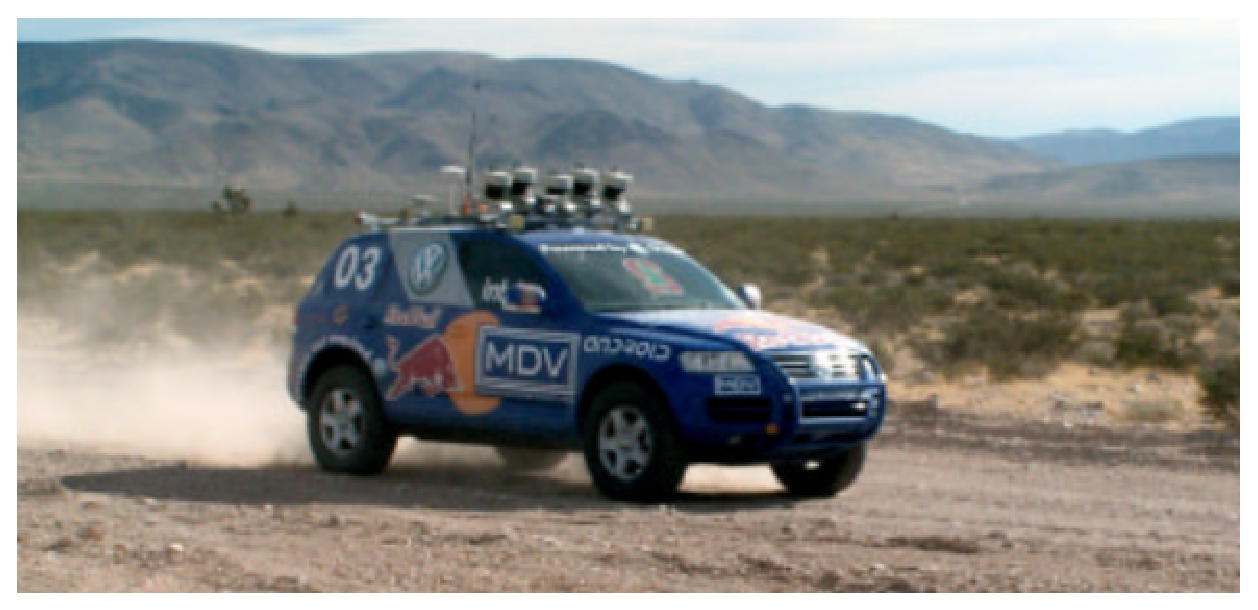
\includegraphics[height=3cm]{imgs/Stanley.eps}
		}
		\subfloat[\label{subfig:boss}]{%
			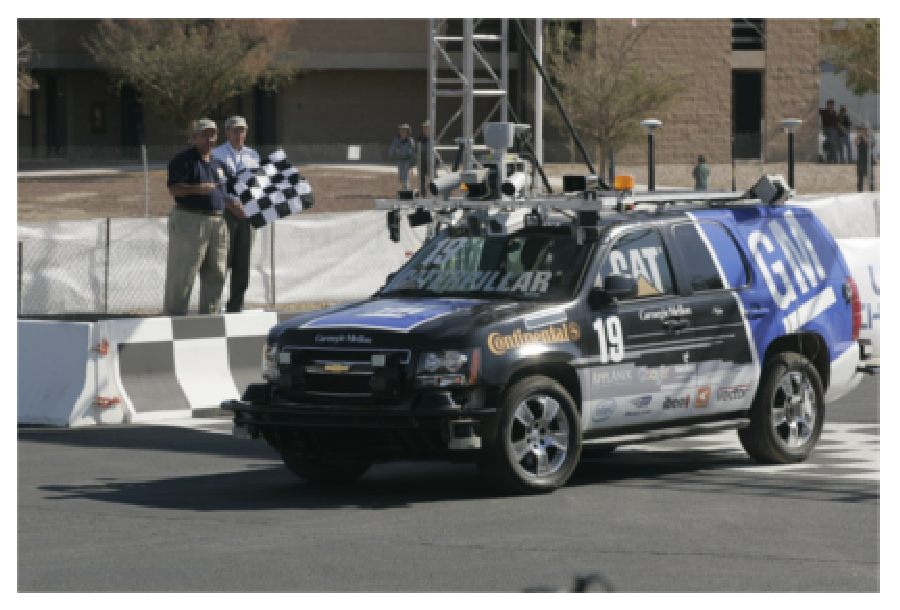
\includegraphics[height=3cm]{imgs/Boss_DARPA_urban_challenge.eps}
		}
	}
	\caption{The winning robots from the 2005 \ac{DARPA} Grand Challenge and 2007 Urban Challenge. Fig. \ref{subfig:stanley} shows Stanford's Stanley at the 2005 \ac{DARPA} Grand Challenge (Image from \cite{Thrun2006}), Fig. \ref{subfig:boss} shows Carnegie Mellon's BOSS at the 2007 \ac{DARPA} Urban Challenge (Image from \cite{Urmson.2008}).}\label{fig:darpa_chal}
\end{figure}
Many researchers involved in the winning teams continued their research within Google's self-driving car project, which started in 2009 and evolved into the Spin-Off company Waymo \cite{Waymo} in 2016.
Another research team continuing their efforts after the \ac{DARPA} challenges is the Annieway team \cite{Annieway}.
One of their major contributions is the release and maintenance of the KITTI vision benchmark suite \cite{Geiger2013IJRR}, a publicly available data set containing data from various test drives in the city of Karlsruhe, rural areas as well as highways focusing on providing real world data for vision tasks like stereo, optical flow and 3D object detection and tracking.\\
The main research goal after the \ac{DARPA} Challenges was to develop automated driving with off-the-shelf sensors \cite{Furgale2013}.
As this thesis focuses on environmental modelling in context of autonomous driving, this section presents research from this field like road detection and modelling (Sec. \ref{subsec:lane}), object detection (Sec. \ref{subsec:obj_detect}) and tracking (Sec. \ref{subsec:obj_track}) as well as sensor fusion (Sec. \ref{subsec:sensor_fusion}) while other aspects like localization \cite{Levinson2010, Thrun2005}, path planning (\todo{citation}) and motion control (\todo{citation}) are neglected.
\subsection{Knowledge Representation}
\label{subsec:knowledge_representation}
Since highly automated vehicles are multi-sensory systems, current automotive world models use mostly probabilistic approaches and Bayesian filtering.
The main difference is the level, at which sensory data is combined \cite{Elfring2016}.
Low-level resp. high-level fusion systems combine raw sensor data e.g. in an occupancy-grid \cite{Tanzmeister2014} or fuse preprocessed object-lists \cite{Elfring2016} respectively.
The work closest to our approach is \cite{Yamazaki2016}, where they use symbolization, a language modelling technique, to obtain semantic descriptions of driving scenes.
% For the specific task of recognizing the current driving context, there have been early approaches using statistical pattern recognition based solely on the ego-vehicle's dynamics \cite{Engstrom2001} or on fusion with camera data \cite{Hauptmann1996}.
% The key difference to previous work is that our approach employs cognitive modelling techniques, which allows us to use symbolization as well, but also to combine it with the benefits of neural networks.
\subsection{Object Detection and Classification}
\label{subsec:obj_detect}
\subsection{Behaviour Analysis}
\label{subsec:behav_analysis}
\section{Cognitive Modeling}
\subsection{Vector based approaches}
\todo{insert context on vector based approaches, different instantiations of \acp{VSA}}\\
\todo{mention \acp{SDR} and \ac{HTM} and related technology from companies like Numenta, cortical}\\
\todo{context on vector based approaches}\\
\todo{briefly explain other applications like natural language processing, word2vec etc.}
\subsection{Symbolic approaches}
\section{Summary}